\chapter{Tree assignment and tracking results} \label{chpt:treeassign}
Our cell tracking method needs to generate a bipartite matching \cite{mosig2009tracking, Xiao:2011} between consective component trees, which performs the role of both cell segmentation and cell association. In the most general form, generalizations of bipartite matching to trees have recently been shown to be $\mathcal{NP}$-hard\cite{canzar2011tree}.
In this thesis, we introduced two types of tree assignment problems. One is tree assignment between component trees, the other is tree assignment between neuron trees. Both models can be implemented by integer linear programming(ILP) and dynamic programming(DP). The two types of solution have different running time which depends on the complexity of tree structure. The tree assignment between trees with each node of few child nodes, such as component tree, is suitable to use DP, otherwise it is suitalbe to use ILP.

\section{Component tree assignment}
\subsection{Problem formulation}
Let $T_1$ and $T_2$ denote two rooted unordered trees, with vertices $U$ and $V$, respectively.  We refer to the set of all possible assignments between $T_1$ and $T_2$ as match $(T_1,T_2) =\Big\{M \subset U \times V | M = \{(u_1,v_1),\ldots,(u_k,v_k)\}\Big\}$. Given a weighting function $w:U\times V \to \mathbb{R}_{\le 0}$, we can assign a weight $W(M) := \sum_{u,v)\in M}w_{u,v}$ to an assisnment $M \in$ match$(T_1,T_2)$. Putting things together, this allows us to define the \emph{tree assignment problem}, which is to find the maximum weighted tree assignment $M$, given $T_1,T_2$ and $w$. The tree assignment problem is a generalization of maximum weighted bipartite matching problem.
\subsubsection{Three points condition}
We deal with tree assignments under \emph{three points condition} for component tree assignment base cosegmentation, which introduces a restriction on the topology of trees with three leaves. We adapt the recursions for the constrained tree edit distance to solve the restricted tree assignment problem.

The three-point condition involves the lowest common ancestor of two vertices $a,b$ in a tree, which we denote by lca$(a,b)$. Now, we defined the tree assignment matching $M \in$ match$(T_1,T_2)$ if for any tree assignments $(a_1,a_2),(b_1,b_2),(c_1,c_2) \in M$, we have
$$
lca(a_1,b_1) \preceq lca(a_1,c_1)  \Rightarrow lca(a_2,b_2) \preceq lca(a_2,c_2)
$$

Intuitively, the three-point condition ensures that for any tree pairs of vertices in an assignment, the topology of the two induced subtrees are in the same heirarchical order.  
\subsubsection{Component tree}
The component tree maintains the inclusion relationship between all possible connected component under all different threshold segmentation. Najman et al.\cite{Najman:04} introduced a quasi-linear algorithm to construct the component tree. And I introduced a pruning principle to simpify the component tree structure (see Chapter\ref{chpt:cptree}).

\subsubsection{Component tree weights}
The weight between two component nodes is defined as the ratio of overlapping size and union size. I introduced a quasi-linear dynamic algorithm to compute all the weights between two component trees (see Sec\ref{sec:cptree-weight}).
\subsection{Integer linear programming (ILP)}
Given two trees $T_1$ and $T_2$, to satisfy the \emph{three point condition}, we introduce the match $M \in$ match$(T_1,T_2)$ such that for any two distinct indices $1 \le i,j \le k$, neither $u_i$ is an ancestor/descendant of $u_j$ nor $v_i$ is an ancestor/descendant of $v_j$. 

For each vertex $u \in T_1, v \in T_2$, introduce binary variable $X_{uv}$, where $X_{uv} = 1$ iff $u$ is assigned to $v$, otherwise $X_{uv} = 0$. For any node $u, u' \in T_1$ and $v, v' \in T_2$, we can define the integer linear model with constraints,
\begin{equation}
\label{eqn:cptree-ilp-st}
\left\{
\begin{array}{l}
X(u,v) \in \{0,1\} \\
\forall u \preceq u', X(u,v) + X(u',v') \le 1 \\
\forall v \preceq v', X(u,v) + X(u',v') \le 1 
\end{array}
\right.
\end{equation}
and the objective function by maximum the sum of weight function,
\begin{equation}
 \max \sum_{u\in T_1, v \in T_2} w(u,v)X(u,v)
\end{equation}

For the constraints \ref{eqn:cptree-ilp-st}, the first constraint ensures the binary values for assignment variable, the second and third constraint ensure that only one node is matched in a leaf-node-to-root-node path in both trees (see Fig\ref{fig:treeassign-cptree}A and Fig\ref{fig:treeassign-cptree}B). 

Let $L(T)$ denotes all the leaf nodes of T; $root(T)$ denotes the root node of tree $T$; $path(u,v) = \{u_1 = u,u_2, \ldots, u_{n-1}, u_n = v\}$ denotes the path from node $u$ to node $v$; $P(T) = \{path(u, root(T))|u \in L(T)\}$ denotes all the leaf-node-to-root-node paths. The above constraints \ref{eqn:cptree-ilp-st} can be re-written as,
\begin{equation}
\left\{
\begin{array}{l}
X(u,v) \in \{0,1\} \\
\forall p \in P(T_1), \sum_{u\in p}\sum_{v \in T_2} X(u,v) \le 1 \\
\forall p \in P(T_2), \sum_{u\in T_1}\sum_{v \in p} X(u,v) \le 1 
\end{array}
\right.
\end{equation}

\subsection{Dynamic programming algorithms (DP)}


Jiang \cite{Jiang:95} provided a less constraint tree assignment algorithm.
For each $A \subseteq \{u_1,u_2,...,u_m\}$, $u_i \in T_1$ and each $B \subseteq \{v_1,v_2,...,v_n\}, v_j \in T_2$. \\
\begin{eqnarray} \label{eqn:lcdp-formular}
W(A,B) = \max \begin{cases}
\max_{a_i \in A, b_j \in B}(W(A-\{a_i\}, B-\{b_j\}) + w(a_i,b_j))\\
\max_{a_i \in A, B' \subseteq B}(W(A-\{a_i\}, B-B') + W(C(a_i), B')) \\
\max_{A' \subseteq A, b_j \in B}(W(A-A', B-\{b_j\}) + W(A', C(b_j))
\end{cases} 
\end{eqnarray}

Assume $r_1$ the root node of $T_1$ and $r_2$ the root of $T_2$, the solution of tree assignment will be $W(C(r_1), C(r_2))$.
Obviously the constrained tree assignment in section \ref{sect:tree-assignment} is covered as a special case by applying the first case of Eqn.\eqref{eqn:lcdp-formular}. 

\begin{figure}[htbp]
\centering
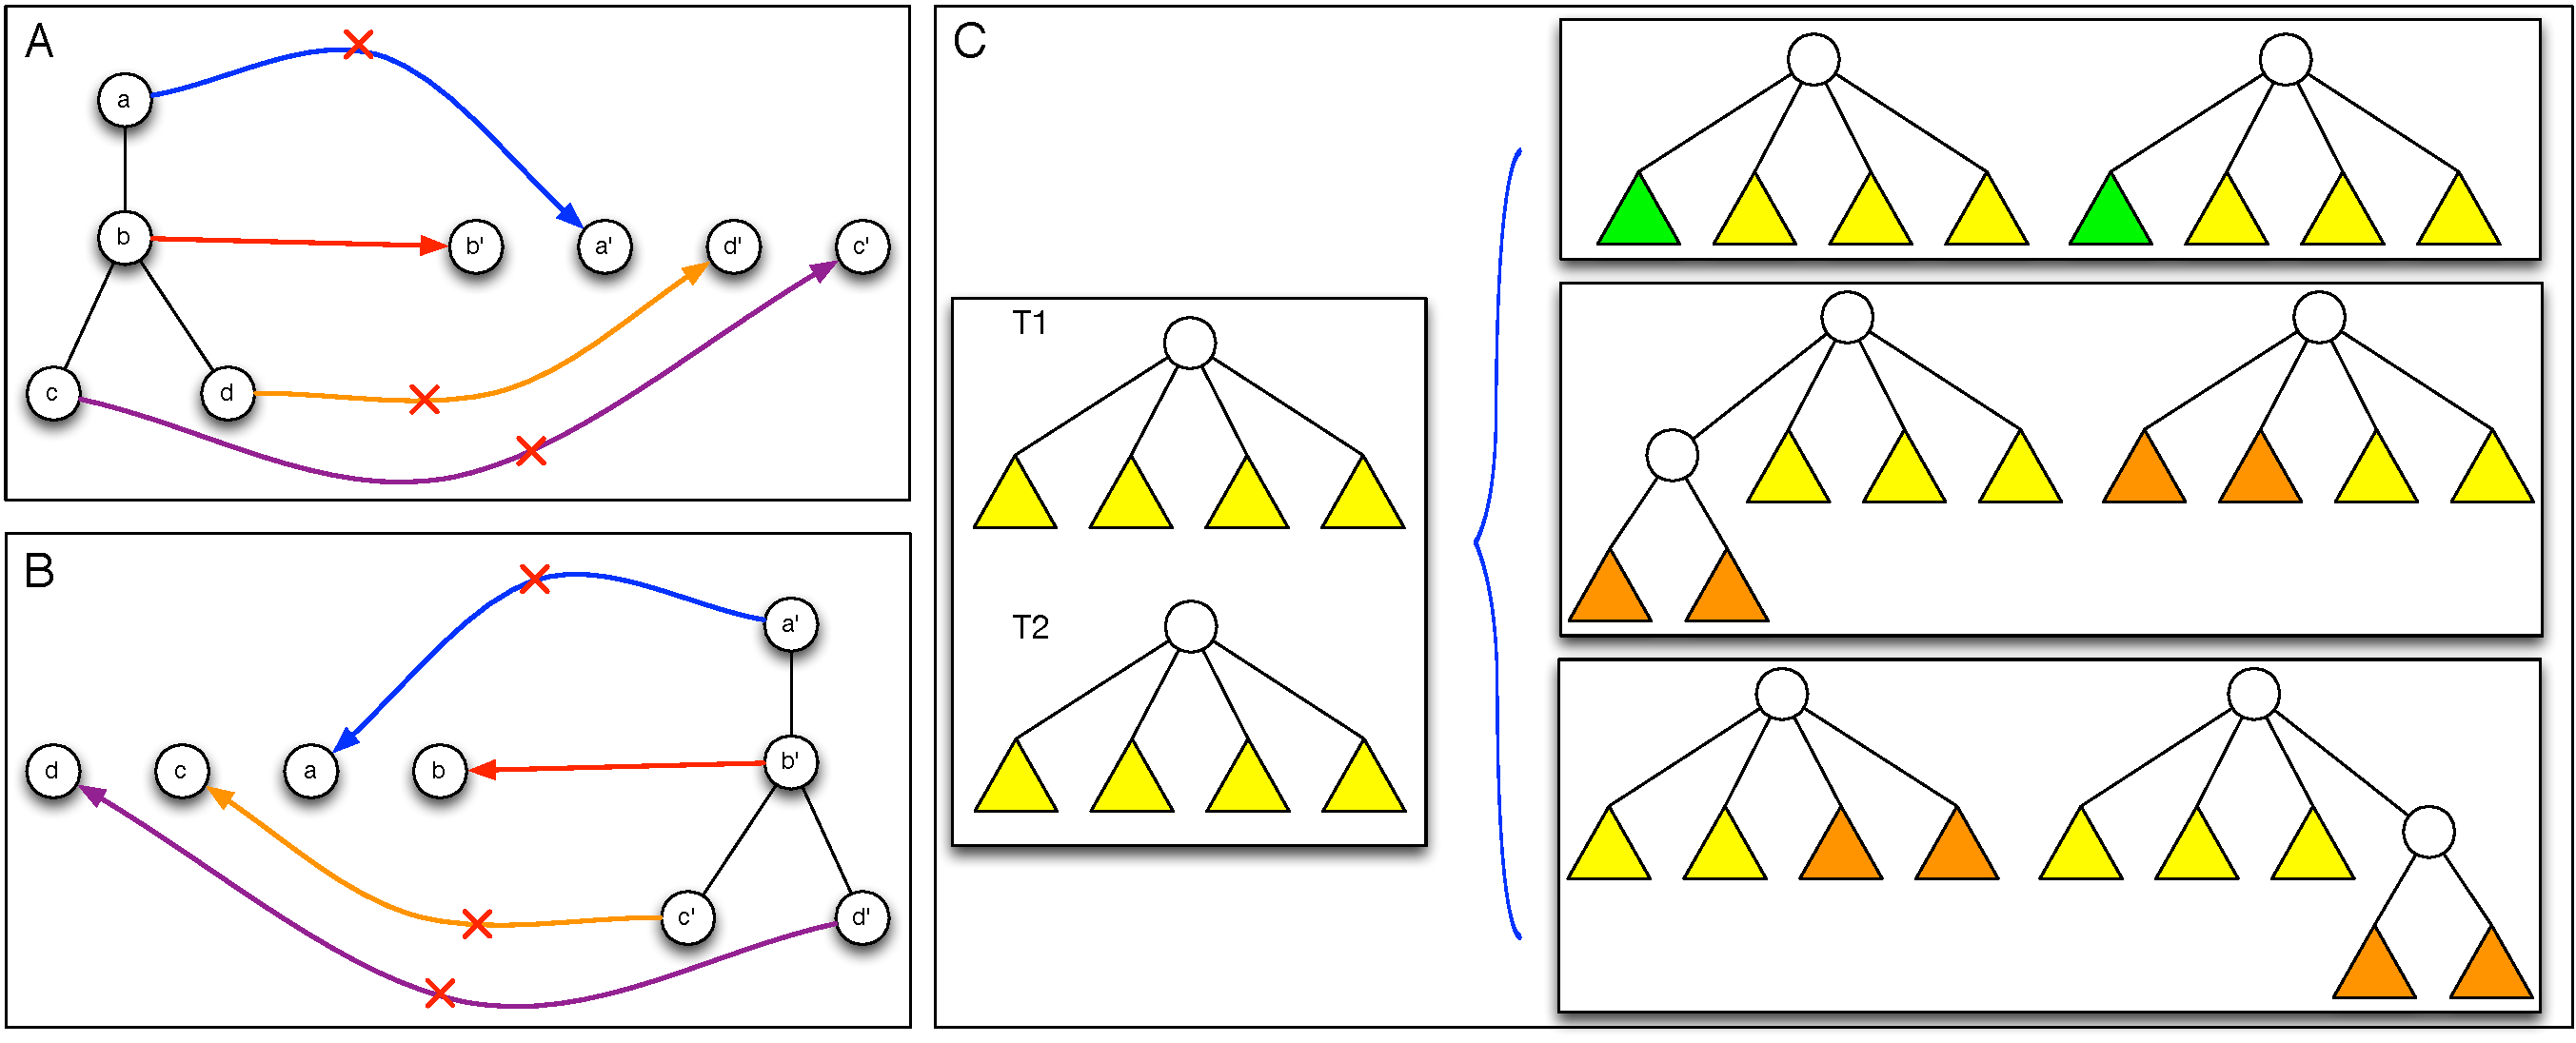
\includegraphics[width=1.0\textwidth]{images/treeassign_cptree}
\caption[ILP and DP models for component tree assignment]{ILP and DP models for component tree assignment. A. The second constraint in ILP model \ref{eqn:cptree-ilp-st} for component tree assignment; B. The third constraint in ILP model \ref{eqn:cptree-ilp-st} for component tree assignment; C. The DP model of component tree assignment.}
\label{fig:treeassign-cptree}
\end{figure}

\subsubsection{Running time}
With the less constrained recurrence, we will get much better result with higher mapping score. However, the time complexity turns out to depend exponentially on the maximum degree of the two trees
\begin{equation*} \label{eqn:lcdp-time}
O\left(\sum_{u_i \in T_1, v_j \in T_2}(2^{|C(u_i)|}\cdot 2^{|C(v_j)|})\right).
\end{equation*}
For binary trees, the running time will be
$O(|T_1|\cdot|T_2)$. \\
For component trees, the runing time will be 
$O\left(2^{|C(r_1)|}\cdot2^{|C(r_2)|}\right)$. \\
\subsubsection{Improvement}
Firstly we define the overlap between $A$ and $B$. We mean $A$ and $B$ have overlap that there exists some element in $A$ ovelaping with some element in $B$, otherwise no overlap.\\ 
When dealing with tree-assignments involving component trees, note that in practice many $A$ and $B$ have no overlap, or only few elements in $A$ overlap with few elements in $B$. The non-overlaping A and B can be neglected in the assignment. The overlaping A and B can be decomposed into disjoint subsets $A=A_0 \cup \ldots \cup A_n$ and $B = B_0 \cup \ldots \cup B_n$ such that $A_1 \cup B_1, \ldots, A_n \cup B_n$ are the connected components in graph $G(V, E)$ , that $V = A \cup B$ and $E = \{(a,b)|a \in A, b \in B, \beta(a) \cap \beta(b) \neq \emptyset\}$,  and $A_0$ and $B_0$ are the collection of isolated nodes of $A$ and $B$. As $A_0$ and $B_0$ can be neglected in the assignment, we have 
\begin{equation*} \label{eqn:ldcp-decomp}
W(A,B) = \sum_{k=1,\ldots,n}{W(A_k, B_k)}
\end{equation*}
In practice, $|A_k|$ and $|B_k|$ will be much smaller than $|A|$ and $|B|$, the runing time will be much smaller, which speed up the algorithm significantly on many instances.
\subsection{Difference between ILP and DP models}
Integer linear programming (ILP) and dynamic programming (DP) provide two different implementations for component tree assignment. DP model implements exactly the three point condition, three point condition fits the ILP model. However, ILP model doesn't always fit three point condition. Fig\ref{fig:treeassign-threepoint}A illustrates the match result in ILP which doesn't fit the three point condition. Fig\ref{fig:treeassign-threepoint2} shows the match difference between ILP and DP, where the segmentation results if ILP contain that of DP.

\begin{figure}[htbp]
\centering
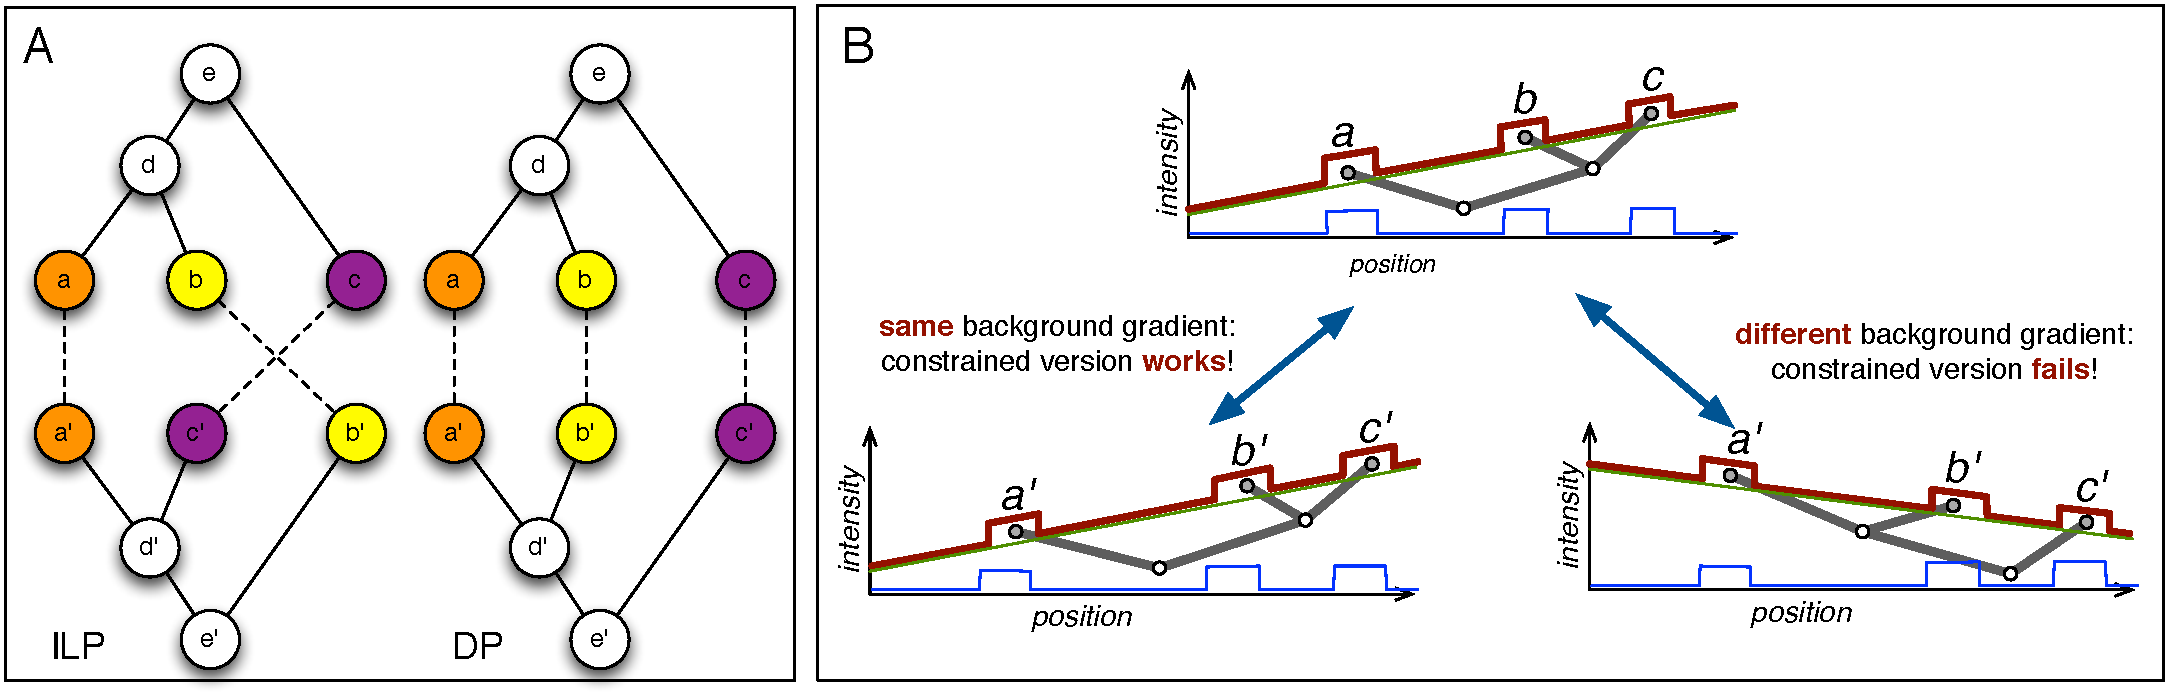
\includegraphics[width=1.0\textwidth]{images/treeassign_threepoint}
\caption[Three point condition]{A. The difference between ILP and DP models, where DP fits exactly three point model, while ILP extends three point condition; B. The explaination of three point condition which is especially efficient when background gradient.}
\label{fig:treeassign-threepoint}
\end{figure}

\begin{figure}[htbp]
\centering
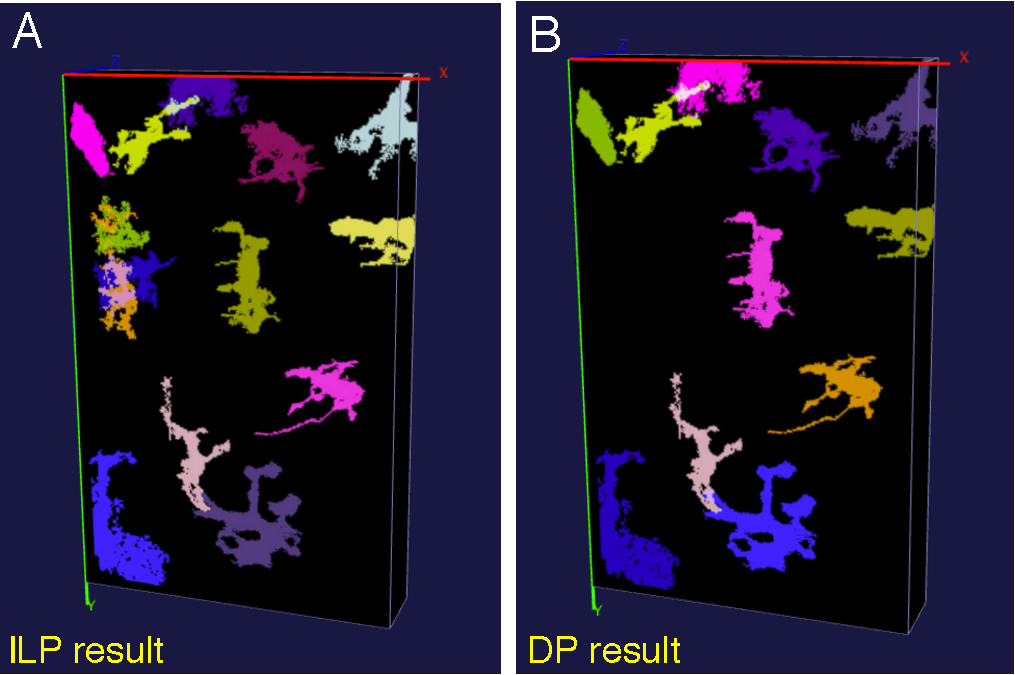
\includegraphics[width=1.0\textwidth]{images/treeassign_threepoint2}
\caption[ILP and DP result difference for microglia cell segmentation]{ILP and DP result difference for microglia cell segmentation, the red circles indicate the additional match result of ILP model.}
\label{fig:treeassign-threepoint2}
\end{figure}

\subsection{A model for cell spliting and merging}
The proposed algorithms can only track the movement of cell without cell splitting and cell merging, as the algorithms descirbed above assign the node in one tree to exactly only one node in the other tree. Both ILP model and DP model will loose the track of cells if cell splitting or cell merging exist. (Usually only cell splitting exists in practice.) We improve the linear tree assignment model that each node in one tree can be assigned to many nodes in the other tree. However, the constraint that only one node is assigned in a leaf-to-root-node path is kept. 

Given two trees $T_1$ and $T_2$, for each vertex $u \in T_1$, $v \in T_2$, we introduce additional two binary variables $Y_u$ and $Z_v$ besides $X_{uv}$. $X_{uv} = 1$ if node $u$ is assigned to node $v$, otherwise $X_{uv} = 0$. If node $u$ is assigned to any node in $T_2$, $Y_u = 1$; and $Y_u = 0$ if node $u$ is not assigned. The same rule works for $Z_v$. The relationship between $Y_u$,$Z_v$ and $X_{uv}$ is given by,
\begin{equation}
	Y_u = 
	\left\{
	\begin{array}{cc}
		0 & \text{if \quad $\sum\limits_{v \in T_2}X_{uv} = 0$} \\
		1 & \text{if \quad $\sum\limits_{v \in T_2}X_{uv} \ge 1$}
	\end{array}
	\right.
	\quad \text{for $u \in T_1$}
\end{equation}
\begin{equation}
	Z_v = 
	\left\{
	\begin{array}{cc}
		0 & \text{if \quad $\sum\limits_{u \in T_1}X_{uv} = 0$} \\
		1 & \text{if \quad $\sum\limits_{u \in T_1}X_{uv} \ge 1$}
	\end{array}
	\right.
	\quad \text{for $v \in T_2$}
\end{equation}
By considering the condition that only one node is assigned for a leaf-node-to-root-node path, the integer linear model is given by
\begin{equation}
\left\{
\begin{array}{l}
\sum\limits_{u \in P1 \in P(T_1)}Y_u \le  1 \\
\sum\limits_{v \in P2 \in P(T_2)}Z_v \le  1 
\end{array}
\right.
\end{equation}
with the same objective function
\begin{equation}
max\sum\limits_{i \in T_1}\sum\limits_{j \in T_2}w_{ij}X_{ij}
\end{equation}

The constraints for $Y_i$ and $Z_j$ is not clear, which seems like a non-linear interger programming. However there are two kinds of methods to define $Y_i$ and $Z_j$ and turn the problem into linear integer programming.

\textbf{Method 1:}
\begin{eqnarray}
\frac{\sum_{v \in T_2}X_{uv}}{|T_2|} \le Y_u \le \sum_{v \in T_2}X_{uv} & \text{for $u \in T_1$} \\
\frac{\sum_{u \in T_1}X_{uv}}{|T_1|} \le Z_v \le \sum_{u \in T_1}X_{uv} & \text{for $v \in T_2$}
\end{eqnarray}
Obviously when $\sum\limits_{u \in T_1}X_{uv}$ equals to zero, $Y_u$ will less than zero, due to the \{0,1\} constraint, $Y_u$ will be zero. When $\sum\limits_{u \in T_1}X_{uv}$ larger than zero,beacuse of $\sum\limits_{u \in T_1}X_{uv}$, $Y_v$ always no greater than $|T_1|$, $Y_u$ will larger then a value, which is larger then zero and no greater than 1. So $Y_u$ will of course be one. This contrains fit the definition of $Y_u$ very well. The contraint also fit to $Z_v$ very well.

\textbf{Method 2:}
\begin{eqnarray}
Y_u \ge X_{uv} &\text{for each $v \in T_2$, for $u \in T_1$}\\
Z_v \ge X_{uv} & \text{for each $u \in T_1$, for $v \in T_2$}\\
\label{con:multi-align1}
Y_u \le \sum\limits_{u \in T_1}X_{uv}  & \text{for $u \in T_1$}\\
\label{con:multi-align2}
Z_v \le \sum\limits_{v \in T_2}X_{uv}  & \text{for $v \in T_2$}
\end{eqnarray}
Once node $u \in T_1$ and node $v \in T_2$ is matched, $X_{uv}$ will be one, and $Y_u$ and $Z_v$ will be no less than $X_{uv}$, so $Y_u$ and $Z_v$ both will be 1. The constraints \ref{con:multi-align1} and \ref{con:multi-align2} is used for nonmatching instances. If node $u \in T_1$ or node $v \in T_2$ is not matched at all, $Y_u$ or $Z_v$ will be 0 either. So now the method 2 fit the definition of $Y_u$ and $Z_v$ perfectly.

\section{Neuron tree assignment}
\subsection{Two points condition}
\subsection{Optimization formula}
\subsection{Integer linear programming}
\subsection{Dynamic programming algorithms}
\section{Cell Tracking results}
